\section{Intro}

Synergy lets you easily share your mouse and keyboard between multiple
computers on your desk, and it's Free and Open Source. Just move your
mouse off the edge of one computer's screen on to another. You can even
share all of your clipboards. All you need is a network connection. Synergy
is cross-platform (works on Windows, Mac OS X and Linux).

\begin{figure}[H]
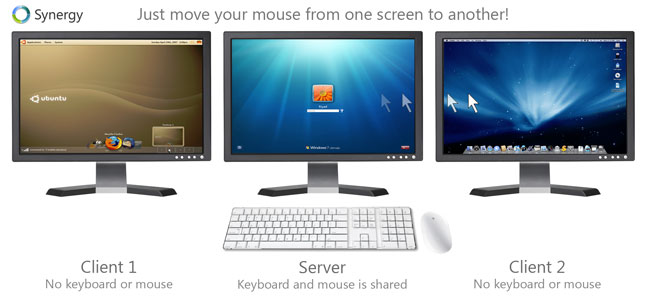
\includegraphics[scale=.65]{graphics/intro.jpg}
\end{figure}

This user guide is written for Synergy version 1.4 -- please upgrade if
you are using an older version (like 1.3). To find your version, click
the "Help" menu, and select "About" or "About Synergy".

More information and download links can be found at our website:
http://synergy-foss.org